\documentclass[11pt]{article}
\usepackage[final]{acl}

\usepackage{times}
\usepackage{latexsym}
\usepackage[T1]{fontenc}
\usepackage[utf8]{inputenc}
\usepackage{microtype}
\usepackage{graphicx}
\usepackage{booktabs}
\usepackage{amsmath}
\usepackage{url}

\title{Whose Robots.txt? Consent-Infrastructure Inequality Across the\\Languages of Web Corpora}

\author{
Austin Cheng\textsuperscript{*} \quad Gary Zhang\textsuperscript{*} \\
William A. Shine Great Neck South High School \\
\texttt{austincheng98@gmail.com} \quad \texttt{zhanggary607@gmail.com} \\
\textsuperscript{*} Equal contribution.
}

\begin{document}
\maketitle

\begin{abstract}
Website owners increasingly restrict AI crawlers through robots.txt and consent-respecting corpus builders honor these signals, but existing audits cover English-centric corpora and report no results stratified by the language served. We measure AI-crawler opt-out for 4,900 domains sampled from the FineWeb and FineWeb-2 subsets of fourteen languages across three resource tiers. The gradient is steep at the domain level, where our sampling design supports it: reachable high-tier domains block at 28.8\% against 11.2\% and 9.8\% for the mid and low tiers, and an exact permutation over the language partition puts the high--low gap at $p = 0.008$. It decomposes cleanly, since whether a robots.txt names any AI agent falls from 33.6\% to 10.6\% across tiers while blocking a named agent shows no tier ordering, and among files already curating a conventional-crawler list the share also naming an AI agent falls from 64.0\% to 19.0\%, which a diffusion account predicts and a maintenance-budget account does not. Under today's robots.txt applied retroactively to a corpus crawled earlier, design-weighted document mass behind a Common Crawl opt-out is 31.2\% for English, with tier means of 26.5\%, 8.9\%, and 10.7\% that put the low tier above the mid tier. Reachability follows the same slope, 78\% of English domains answering a request against 39\% for Uyghur. What differs across these fourteen subsets is recorded policy, and a consent-respecting rebuild would filter high-resource text more heavily than the rest. We release every fetched robots.txt, the derived rates, and the code.\footnote{\nolinkurl{https://github.com/austincheng98/robots-txt}}
\end{abstract}

\section{Introduction}

The web is closing to AI crawlers: \citet{longpre2024consent} found that 28\% of the most actively maintained sources behind C4, RefinedWeb, and Dolma now restrict AI agents through robots.txt, up from near-zero twelve months earlier. Corpus builders honor these signals, making robots.txt an operational consent layer for pretraining data.

Prior audits do not stratify by language. Writing an AI clause into robots.txt requires knowing that GPTBot exists, maintaining a server configuration, and following a policy debate conducted in English. If those preconditions concentrate in wealthy, English-speaking web infrastructure, recorded opt-out should fall with the resource level of the language a domain serves, so filtering by robots.txt may remove recorded refusals rather than preferences.

We test this prediction using FineWeb \citep{penedo2024fineweb} and FineWeb-2 \citep{penedo2025fineweb2}, which ship source URLs for every document. We sample 350 domains per language in two stages, fetch each live robots.txt, and parse fifteen AI crawlers. Domain-level rates are primary; composition estimates carry a weaker Horvitz--Thompson correction. The question is whether the gradient is in naming an AI agent, survives size and site-type controls, and changes the composition a consent-respecting rebuild would inherit.

\section{Related Work}

\citet{longpre2024consent} provides the longitudinal, English-centric baseline; we add per-language consent results. \citet{dodge2021documenting} shows how corpus construction can alter composition, while \citet{steinacker2025misinformation,cui2025odyssey} show that crawler restrictions vary across site populations and bot rosters, without a language breakdown. The underlying protocol began as an informal convention between crawler operators and site owners \citep{koster1994standard}. FineWeb-2 supplies our per-document URL frame \citep{penedo2025fineweb2}; multilingual data-quality work asks what pipelines admit \citep{kreutzer2022quality,caswell2020langid}, whereas we ask who can keep text out.

\section{Method}

\subsection{Sampling}

We take fourteen language subsets across three resource tiers: English, German, Japanese, and French (high); Indonesian, Turkish, Vietnamese, Thai, and Azerbaijani (mid); Swahili, Sundanese, Yoruba, Uyghur, and Irish (low). Tiers track \citet{joshi2020state}: every high-tier language is class 5, every low-tier language classes 1--2, and the mid tier classes 3--4 apart from Azerbaijani (class 1), whose placement we test in Section~\ref{sec:results}. English comes from FineWeb \texttt{sample-10BT} and the other thirteen from FineWeb-2, which has no English subset; both derive from Common Crawl through near-identical pipelines, but English's census is nonetheless drawn from a differently filtered corpus. We stream up to 200,000 documents per subset (the cap binds everywhere except Sundanese, Yoruba, and Uyghur) and aggregate document and token counts by domain. Our domain unit is the URL hostname with a leading \texttt{www.} stripped, not the registered domain or eTLD+1, so a publisher network spread over regional subdomains contributes several units. Frame membership comes from the pipeline's own language identification, so multilingual hosts appear under more than one language and language-ID error enters our frame \citep{caswell2020langid}.

The census retains the top 20,000 domains by document mass and discards the rest before sampling. The cap binds for all four high-tier languages, four of the five mid-tier ones, and no low-tier one, discarding 117,447 English and 82,783 Japanese domains, so every estimate below is for the top-20,000-domain web of a language, a population systematically narrower for the high tier. Within it we draw 350 domains in two stages, the top 175 by document mass with certainty and 175 uniformly at random from the remaining $N-175$. The tail weight varies six-fold, from 18.7 for Uyghur to 113.3 for English, so simply adding the mass of sampled domains, as an earlier version did, gives every head domain the weight of a tail domain and describes the sampled head rather than the language. Every mass-weighted quantity below is instead a Horvitz--Thompson estimate, defined in the caption of Table~\ref{tab:app-mass}. Domain-level rates carry no weights, and the two stages double as a size control.

\subsection{Parsing}

We fetch \texttt{https://domain/robots.txt} with an 8-second timeout, falling back to HTTP, and archive every response body. We parse user-agent blocks for fifteen AI-associated crawlers (GPTBot, CCBot, ClaudeBot, Google-Extended, Bytespider, and ten more), recording a full opt-out when an agent receives \texttt{Disallow:~/}; a domain counts as opted out when it fully blocks at least one. We also record whether a file names any of the fifteen in any rule including \texttt{Allow} rules, which factors opt-out into naming an AI crawler and blocking a named one. Relabeling a stratified sample of 60 archived bodies by hand reproduces the parser verdict in 58, an agreement of 96.7\%, the two disagreements running in opposite directions: \texttt{nli.ie} gives Bytespider a \texttt{Disallow:~*} rather than a literal slash, which our rule excludes and the manual label counts as a block, and \texttt{pleinelune.niceboard.com} has a body truncated at 6,000 characters inside an old-style scraper blocklist, so the parser records a block the visible text cannot support. Domain-level rates carry 2,000-draw bootstrap intervals.

\subsection{Policy}

Both corpora derive from Common Crawl, so the restriction a rebuild would be bound by is the one addressed to CCBot, which we report as the rebuild policy alongside the fifteen-agent union as the broader ``any AI agent'' reading, GPTBot-only, and two variants folding in a blanket \texttt{User-agent:~*} with \texttt{Disallow:~/} (Table~\ref{tab:app-policy}). Since tier is assigned at the language level, domains within a language are not independent under a tier-shuffle null, so our primary test is an exact permutation over the language partition (126 high-versus-low splits), equal-weighted unless we say otherwise; domain-pooled shuffles overstate precision and serve as descriptives only.

Live robots.txt records policy today while the corpora were crawled earlier, so every composition number below is what today's robots.txt would do to an earlier crawl and not a forecast of a future crawl, the frame of \citet{longpre2024consent}. Unreachable domains are reported rather than dropped, since reachability itself tracks the infrastructure gap under study.

\section{Results}
\label{sec:results}

\begin{table}[t]
\centering
\scriptsize
\setlength{\tabcolsep}{3pt}
\begin{tabular}{lcccccc}
\toprule
Language & Reach & Names & Opt-out [95\% CI] & Mass & $n$ & Blk \\
\midrule
\multicolumn{7}{l}{\emph{High tier}}\\
English & .78 & .493 & .467 [.408, .529] & .392 & 134 & .95 \\
German & .73 & .402 & .299 [.244, .354] & .426 & 102 & .75 \\
French & .77 & .264 & .230 [.182, .279] & .271 & 71 & .87 \\
Japanese & .65 & .159 & .128 [.088, .173] & .143 & 36 & .81 \\
\multicolumn{7}{l}{\emph{Mid tier}}\\
Indonesian & .64 & .276 & .138 [.093, .187] & .084 & 62 & .50 \\
Thai & .61 & .168 & .126 [.084, .173] & .163 & 36 & .75 \\
Turkish & .68 & .214 & .109 [.071, .147] & .088 & 51 & .51 \\
Azerbaijani & .63 & .131 & .104 [.068, .144] & .095 & 29 & .79 \\
Vietnamese & .61 & .089 & .080 [.047, .113] & .062 & 19$^\dagger$ & .89 \\
\multicolumn{7}{l}{\emph{Low tier}}\\
Sundanese & .47 & .129 & .123 [.074, .178] & .077 & 21 & .95 \\
Yoruba & .43 & .113 & .113 [.066, .166] & .154 & 17$^\dagger$ & 1.00 \\
Uyghur & .39 & .109 & .109 [.058, .167] & .123 & 15$^\dagger$ & 1.00 \\
Irish & .58 & .124 & .104 [.064, .149] & .123 & 25 & .84 \\
Swahili & .58 & .064 & .054 [.025, .089] & .094 & 13$^\dagger$ & .85 \\
\bottomrule
\end{tabular}
\caption{AI-crawler opt-out by language. Reach is the share of 350 sampled domains answering robots.txt; Names and Opt-out are, among reachable domains, the shares naming at least one of fifteen AI agents and fully blocking one, respectively; bracketed intervals are bootstrap 95\% CIs. Mass is design-weighted document mass behind a fifteen-agent block under today's robots.txt applied retroactively; $n$ counts reachable domains naming an agent and Blk is the share of them blocking one. $^\dagger$ marks $n < 20$, where Blk is a count.}
\label{tab:main}
\end{table}

\subsection{Consent}

English sits alone at the top of Table~\ref{tab:main} with 46.7\% of reachable domains blocking at least one AI crawler, German next at 29.9\%. Pooled within tiers, reachable high-tier domains block at 28.8\% ($n=1{,}021$) against 11.2\% ($n=1{,}112$) and 9.8\% ($n=857$), a 19.0-point high--low gap with cluster permutation $p = 0.008$ equal-weighted and $0.032$ count-weighted, and the English CI $[.408, .529]$ overlaps no mid- or low-tier interval. Taking each language as one unit the tier means are 28.1\%, 11.1\%, and 10.0\%, and testing the high tier against all ten remaining languages widens the reference set to 1,001 splits and sharpens the verdict to $p = 0.002$. The step sits at the high tier, since mid and low are not separable ($p \ge 0.45$), so this is a two-level split rather than a three-way ordering, and tier rank predicts opt-out at $\rho = 0.69$ ($p = 0.009$). None of this is mass-weighted or changes under the design weights below.

Figure~\ref{fig:gradient} summarizes the decomposition. Opt-out factors into whether a robots.txt names any of the fifteen agents and whether a named agent is fully blocked, and only the first step shows the gradient. Pooled naming runs 33.6\%, 17.7\%, and 10.6\%, a 23.0-point high--low gap with cluster $p = 0.008$ ($p = 0.007$ against all ten remaining languages, $\rho = 0.77$, $p = 0.002$), and English alone reaches 49.3\%. CCBot (428 blocks), GPTBot (422), and ClaudeBot (399) lead in every tier (rank correlations 0.89 to 0.94). Conditional on naming, full blocking shows no tier ordering we can detect: 85.7\% (high, $n=343$), 62.9\% (mid, $n=197$), and 92.3\% (low, $n=91$), cluster $p = 0.167$, bootstrap 95\% interval on the pooled gap $[0.6, 13.0]$ points. That is consistent with no ordering rather than evidence of its absence, and the denominators say why: four languages have fewer than twenty naming domains, the 100.0\% cells for Yoruba (17 of 17) and Uyghur (15 of 15) are counts not rates, and the low-tier 92.3\% rests on 91 domains.

\begin{figure*}[t]
\centering
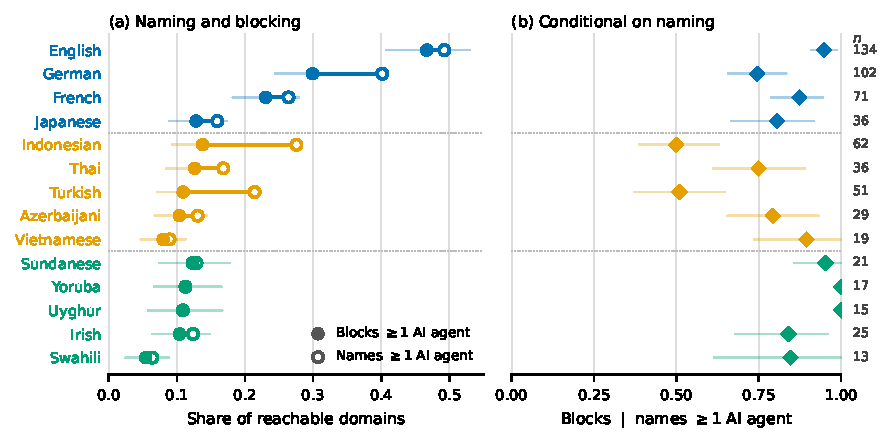
\includegraphics[width=0.55\textwidth]{../figures/fig_gradient_v2.pdf}
\caption{Consent gradient and decomposition. Filled/open markers show blocking/naming rates; panel (b) conditions blocking on naming and labels the naming count $n$. Colors mark tiers.}
\label{fig:gradient}
\end{figure*}

\subsection{Mechanisms}

The mid tier's 62.9\% comes almost entirely from Indonesian and Turkish sites, without which it is 79.8\%, and in both one template rather than a distribution of site-level decisions does the work. Of the 31 Indonesian domains naming an agent without blocking it, 28 are regional subdomains of \texttt{tribunnews.com}, whose shared robots.txt places Google-Extended and GPTBot in the same \texttt{Allow:~/} group as Googlebot. Of the 25 Turkish ones, 20 share a news-CMS template that stacks eight AI user-agent lines and then opens a \texttt{User-agent:~*} group of path-prefix disallows, so the named agents receive partial rules rather than \texttt{Disallow:~/}, exactly where recorded policy and preference come apart.

Three mechanisms behind a gap in recorded policy are partly observable. If low-tier operators simply maintain their files less, they should name conventional crawlers less too, and they do not: naming at least one of fifteen conventional crawlers (Googlebot, Bingbot, AhrefsBot, and others) runs 35.7\%, 19.0\%, and 24.6\%, neither monotone nor significant (gap 9.7 points, cluster $p = 0.190$), while AI naming over the same files has $p = 0.008$. Restricting to files that already curate a conventional list, the share also naming an AI agent is 64.0\% (high, $n=364$), 44.5\% (mid, $n=211$), and 19.0\% (low, $n=211$), a 39.7-point gap with cluster $p = 0.008$. A maintenance-budget account predicts both rates fall together and they do not, while diffusion of the AI-agent token set predicts exactly this. The ``aware and permitting'' signal agrees, since files naming an AI agent and blocking none are 4.8\%, 6.6\%, and 0.8\% of reachable domains ($p = 0.008$), essentially absent in the low tier. Two caveats belong here. Low-tier conventional naming is partly inherited, since SEO blocklists for SemrushBot, MJ12bot, and AhrefsBot ship with some templates and dominate the low tier's non-Google entries. And stock CMS defaults are real: an untouched WordPress, Blogger, or Wix body is 25.2\% of the low-tier sample against 9.0\% of the high-tier one. Restricting to files somebody edited, the gradient survives at 33.0\%, 14.1\%, and 13.1\% (cluster $p = 0.016$), so platform defaults are part of the gap and not the whole of it.

Site-type controls point the same way without settling much, since the gradient holds within ccTLDs (31.7\%, $n=432$; 12.2\%, 329; 13.3\%, 181) and within gTLDs (28.4\%, 510; 10.7\%, 707; 9.8\%, 590), and platform-hosted subdomains, 12.0\% of the low-tier sample against 2.1\% of the high-tier one, almost never opt out, yet removing them moves the pooled gap only from 19.0 to 18.4 points, the low tier's non-platform rate of 11.0\% still far below the high tier's 29.4\%. Commercial incentive, legal exposure, and publisher type remain live alternatives our data cannot separate; Table~\ref{tab:app-mech} carries the remaining splits.

\subsection{Composition}

Under today's robots.txt applied retroactively to a corpus crawled earlier, and taking the CCBot restriction a rebuild would be bound by, design-weighted document mass behind a block is 31.2\% for English, with tier means of 26.5\%, 8.9\%, and 10.7\% (cluster $p = 0.032$ high--low, $0.005$ high-versus-rest); the CCBot rate at the domain level is 23.8\%, 9.6\%, and 8.5\% ($p = 0.032$ and $0.007$). Reading ``any AI agent'' instead raises English to 39.2\% of document mass (41.4\% of tokens) and the tier means to 30.8\%, 9.8\%, and 11.4\% on document mass, 27.6\%, 8.7\%, and 11.2\% on tokens; Figure~\ref{fig:estimands} compares these domain and mass estimands. Design weighting materially weakens this part of the paper: under the CCBot policy, as under any-15, the low tier sits above the mid tier on mass, so what survives is a high-tier step and not a three-way gradient; high--low under any-15 gives $p = 0.016$ on document mass but $p = 0.10$ on tokens, which is not significant, while high-versus-rest survives both ($p = 0.003$ and $0.015$), and the rank correlation with tier falls to $\rho = 0.51$ ($p = 0.069$) and $\rho = 0.22$ ($p = 0.45$). The unweighted figures of an earlier version, 62.4\% for English and tier means of 44.3\%, 13.3\%, and 12.2\%, describe the sampled head: the top 175 English domains by mass were fetched with certainty, and 63.9\% of the mass of those that answered sits behind a block. Table~\ref{tab:app-mass} gives per-language mass.

The effect is robust to which AI agent defines the policy and not to folding in a blanket \texttt{User-agent:~*} with \texttt{Disallow:~/}. Wildcard-only blocking runs slightly against the tier order (8.5\%, 9.7\%, and 10.9\% pooled, $p = 0.37$), since low-tier sites use blanket blocks more than AI-specific clauses. Counting one as an opt-out alongside the fifteen agents gives 32.9\%, 13.1\%, and 14.7\%, which still separates high from low ($p = 0.040$) but inverts mid and low, and combining it with the CCBot policy is the one variant where the high--low test fails, at $p = 0.064$, though high-versus-rest survives every variant at $p \le 0.008$. A reader who takes a blanket block to express the same refusal as a named AI clause should read our claim as a high-tier step with no ordering below it.

\begin{figure}[t]
\centering
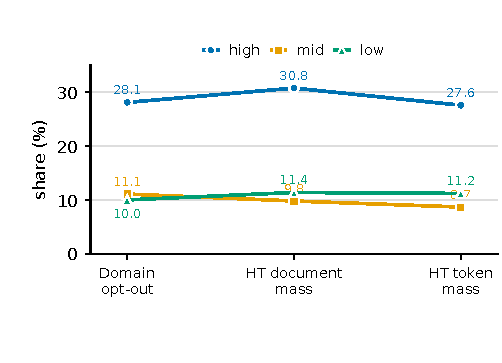
\includegraphics[width=\columnwidth]{../figures/fig_estimands.pdf}
\caption{Tier means under three estimands. Domain opt-out is the reachable-domain rate; design-weighted document and token mass are Horvitz--Thompson estimates under the fifteen-agent policy.}
\label{fig:estimands}
\end{figure}

\subsection{Robustness}

Azerbaijani is Joshi class 1 but sits in our mid tier, and neither correction disturbs anything: excluding it leaves the high--low test at $p = 0.008$, moving it to the low tier strengthens that test to $p = 0.005$, and the rank correlation rises in both cases. Treating a 404 or 410 as an observed policy of no restriction rather than a failed fetch cleans the gradient slightly, with tier means of 25.9\%, 10.3\%, and 8.0\%, high--low $p = 0.008$, and $\rho = 0.76$ ($p = 0.003$).

High-tier samples contain larger publishers and large sites block more, so the gradient could be a size effect, which the two stages check directly. Among the 175 head domains per language, high-tier sites block at 40.4\% ($n=559$) against 10.6\% ($n=538$) in the low tier, cluster $p = 0.008$; among tail domains the rates are 14.7\% ($n=462$) and 8.5\% ($n=319$), pointing the same way but not distinguishable from chance ($p \ge 0.30$), so the tail is not confirmation. A head domain is large only relative to its own language, and the top 175 hold 10.9\% of retained English document mass against 85.9\% of retained Uyghur mass, so this is a within-language stratum control, not a matched comparison.

Between 65\% and 78\% of sampled high-tier domains answer a robots.txt request against 39--58\% in the low tier (cluster $p = 0.008$, $\rho = 0.92$, $p < 10^{-4}$). DNS failure, the domain no longer resolving, rises from 8.9\% of high-tier fetches to 19.9\% and 26.3\% and accounts for roughly half of mid- and low-tier failures, while 403 is flat at 4.6\%, 4.6\%, and 4.5\%. The gradient is therefore more consistent with link rot than with a single cloud vantage point, though geographic blocking remains unmeasured. Per-language failure types are in Table~\ref{tab:app-fail}.

\section{Discussion}

\subsection{Interpretation}

The decomposition and the proxies narrow the space of mechanisms without closing it. Capacity alone does not fit, since conventional-crawler naming shows no significant tier gradient while AI naming among the very files that curate a conventional list falls from 64.0\% to 19.0\%. Deliberate permission does not fit the low tier either, since a web that engaged with AI crawlers and chose to admit them would produce naming without blocking, and that pattern is 0.8\% of low-tier files. Platform defaults are a component and not the whole, since restricting to edited files leaves a gradient at $p = 0.016$. Awareness and infrastructure is the interpretation the evidence best supports, and it remains an interpretation, since we cannot observe the preferences of domains that never mention an AI agent and silence equals neither refusal nor consent. What the data establish is narrower, that the operative consent mechanism transmits a gradient in recorded policy which any filter built on robots.txt inherits. Two designs would settle the rest: surveying low-tier operators, which measures awareness as no file-level proxy can, and a category-matched comparison sampling news sites against news sites across languages, of which our hostname-keyword and TLD splits are the weakest possible version.

Honoring robots.txt beats ignoring it, but treating it as the consent layer privileges the infrastructure-rich web. Corpus builders can act by reporting per-language consent-filtered composition alongside raw composition in every data card, which our release makes cheap for any corpus shipping source URLs.

\section{Limitations}

\subsection{Sampling}

We sample 350 domains per language in two stages from censuses capped at 20,000 domains, so every estimate generalizes to the top-20,000-domain web of a language rather than to its web, and that restriction bites hardest in exactly the languages with the most domains. Mass-weighted quantities depend on a head of 175 domains that a different draw would mostly re-select, and the design-weighted estimates inherit large tail weights, up to 113.3 for English, which makes them noisier than their point estimates suggest. Domain-level rates are the quantity our design supports best and we have made them the headline accordingly. English's census comes from FineWeb rather than FineWeb-2, because FineWeb-2 has no English subset; the pipelines are near-identical and both corpora derive from Common Crawl, but we cannot rule out that the difference contributes to English's position.

\subsection{Measurement}

All fetches issue from one cloud vantage point. The failure-type breakdown argues against this producing the gradient, since 403s are flat across tiers while DNS failures are not, but geo-dependent robots.txt and geo-dependent blocking go unmeasured and the released per-domain failure types let a reader audit this. Language attribution inherits whatever errors the corpus pipeline's language identification makes, and a domain serving several languages can enter more than one frame. Our domain unit is a hostname, so a publisher network spread over regional subdomains contributes many units, which matters most for the conditional-blocking analysis.

Robots.txt is the mechanism corpus builders honor, but preferences can also be recorded in the TDM Reservation Protocol \citep{tdmrep2024}, in \texttt{ai.txt} proposals and \texttt{noai} values in \texttt{robots} meta tags and \texttt{X-Robots-Tag} headers, and in terms of service no crawler parses \citep{longpre2024consent}. All demand the same infrastructure literacy and vendor vocabulary, so we expect them to track the gradient rather than offset it, while CDN-managed AI blocking plausibly cuts the other way.

Our fifteen-agent roster follows current industry practice, but sites can also express preferences in terms of service or use emerging standards we do not parse, and rates under the named-agent criterion are lower bounds on expressed restriction. Expressed restriction is in turn not enforcement, since crawlers comply with robots.txt selectively \citep{kim2025scrapers,liu2024somesite}, so what we measure is the demand to be excluded rather than the supply of compliance. The retroactivity caveat applies throughout: 2026 robots.txt cannot bind crawls that already happened.

\subsection{Scope}

Fourteen languages are not the web and our tiers are coarse. The gradient we report is a statement about the fourteen subsets we sampled, since the language-cluster tests treat those fourteen as the population of interest rather than as a sample drawn from all languages, and nothing here licenses an extrapolation to the roughly 1,800 languages FineWeb-2 covers.

\section*{Ethics Statement}

Our measurement reads only files that site operators publish for automated clients, at one request per domain, and the release contains robots.txt bodies together with the domain names already present in the public FineWeb and FineWeb-2 URL fields. We collect no personal data and no page content. Naming domains that do not block AI crawlers could in principle direct scrapers toward them, but those domains already appear in the public corpora we sample from, so the release adds no exposure the corpora do not already create.

\bibliography{references}

\raggedbottom
\appendix
\setlength{\dblfloatsep}{10pt}
\setlength{\textfloatsep}{10pt}
\setlength{\floatsep}{10pt}
\makeatletter
\setlength{\@dblfptop}{0pt}
\setlength{\@dblfpsep}{10pt}
\setlength{\@dblfpbot}{0pt}
\makeatother
\twocolumn[
\section{Per-language tables}
\label{sec:appendix}

\begin{minipage}{\textwidth}
\centering
\footnotesize
\setlength{\tabcolsep}{4pt}
\begin{tabular}{llrrrrrrr}
\toprule
Language & Tier & census & $N$ retained & dropped & $w_{\text{tail}}$ & head \% of mass & doc mass (unwt.) & doc mass (design-wt.) \\
\midrule
English & high & 137,447 & 20,000 & 117,447 & 113.3 & 10.9 & 62.4 & 39.2 \\
German & high & 54,729 & 20,000 & 34,729 & 113.3 & 36.0 & 52.7 & 42.6 \\
Japanese & high & 102,783 & 20,000 & 82,783 & 113.3 & 33.2 & 23.6 & 14.3 \\
French & high & 59,428 & 20,000 & 39,428 & 113.3 & 31.5 & 38.6 & 27.1 \\
Indonesian & mid & 92,687 & 20,000 & 72,687 & 113.3 & 18.3 & 16.0 & 8.4 \\
Turkish & mid & 51,349 & 20,000 & 31,349 & 113.3 & 38.2 & 14.6 & 8.8 \\
Vietnamese & mid & 67,868 & 20,000 & 47,868 & 113.3 & 28.3 & 8.3 & 6.2 \\
Thai & mid & 68,925 & 20,000 & 48,925 & 113.3 & 24.7 & 17.3 & 16.3 \\
Azerbaijani & mid & 14,838 & 14,838 & 0 & 83.8 & 57.3 & 10.5 & 9.5 \\
Swahili & low & 9,225 & 9,225 & 0 & 51.7 & 68.6 & 11.1 & 9.4 \\
Sundanese & low & 10,339 & 10,339 & 0 & 58.1 & 55.2 & 8.2 & 7.7 \\
Yoruba & low & 5,641 & 5,641 & 0 & 31.2 & 69.3 & 17.4 & 15.4 \\
Uyghur & low & 3,453 & 3,453 & 0 & 18.7 & 85.9 & 10.8 & 12.3 \\
Irish & low & 14,487 & 14,487 & 0 & 81.8 & 54.0 & 13.5 & 12.3 \\
\midrule
\multicolumn{7}{l}{Tier means, document mass} & 44.3 / 13.3 / 12.2 & 30.8 / 9.8 / 11.4 \\
\multicolumn{7}{l}{Tier means, token mass} & 38.8 / 11.7 / 11.1 & 27.6 / 8.7 / 11.2 \\
\bottomrule
\end{tabular}
\captionof{table}{Sample design and composition. Fourteen language subsets contribute 350 domains each across high/mid/low tiers. ``census'' is the pre-cap domain count, $N$ the retained count, $w_{\text{tail}}=(N-175)/175$ the tail weight, and ``head \% of mass'' the share in 175 certainty-selected domains; final columns are unweighted and Horvitz--Thompson design-weighted document mass behind a block.}
\label{tab:app-mass}
\end{minipage}

\vspace{10pt}
\begin{minipage}{\textwidth}
\centering
\scriptsize
\setlength{\tabcolsep}{4pt}
\begin{tabular}{llrrrrrr}
\toprule
Language & Tier & any-15 & CCBot only & GPTBot only & CCBot or \texttt{*} & any-15 or \texttt{*} & \texttt{*} only \\
\midrule
English & high & 46.7 & 40.8 & 38.2 & 44.1 & 49.6 & 9.6 \\
German & high & 29.9 & 25.2 & 24.0 & 34.3 & 39.0 & 13.4 \\
Japanese & high & 12.8 & 8.8 & 10.6 & 11.5 & 15.0 & 4.0 \\
French & high & 23.0 & 20.4 & 17.8 & 23.0 & 25.3 & 6.7 \\
Indonesian & mid & 13.8 & 12.0 & 12.4 & 13.3 & 14.7 & 8.9 \\
Turkish & mid & 10.9 & 8.8 & 10.5 & 11.3 & 13.0 & 8.8 \\
Vietnamese & mid & 8.0 & 7.0 & 7.5 & 8.9 & 9.9 & 8.0 \\
Thai & mid & 12.6 & 10.7 & 10.7 & 13.6 & 15.4 & 11.7 \\
Azerbaijani & mid & 10.4 & 9.5 & 9.9 & 11.7 & 12.6 & 11.3 \\
Swahili & low & 5.4 & 4.9 & 5.4 & 7.4 & 7.9 & 5.4 \\
Sundanese & low & 12.3 & 10.4 & 9.2 & 19.0 & 20.9 & 17.2 \\
Yoruba & low & 11.3 & 9.9 & 7.9 & 13.9 & 15.2 & 10.6 \\
Uyghur & low & 10.9 & 9.4 & 10.1 & 18.1 & 18.8 & 16.7 \\
Irish & low & 10.4 & 7.9 & 9.4 & 10.9 & 13.4 & 7.4 \\
\midrule
Tier means & & 28.1 / 11.1 / 10.0 & 23.8 / 9.6 / 8.5 & 22.7 / 10.2 / 8.4 & 28.2 / 11.8 / 13.9 & 32.2 / 13.1 / 15.2 & 8.4 / 9.7 / 11.5 \\
High vs low $p$ & & 0.008 & 0.032 & 0.008 & 0.064 & 0.040 & 0.37 \\
High vs rest $p$ & & 0.002 & 0.007 & 0.003 & 0.008 & 0.005 & 0.36 \\
\bottomrule
\end{tabular}
\captionof{table}{Domain-level opt-out (\%) over status-200 responses under six crawler policies. CCBot only is the Common Crawl rebuild policy; \texttt{*} is blanket \texttt{User-agent:~*} with \texttt{Disallow:~/}. Tier means are high/mid/low, and $p$-values are exact equal-weighted language-partition permutations.}
\label{tab:app-policy}
\end{minipage}
]

\twocolumn[
\begin{minipage}{\textwidth}
\centering
\footnotesize
\setlength{\tabcolsep}{3.5pt}
\renewcommand{\arraystretch}{0.88}
\begin{tabular}{llrrrrrrr}
\toprule
Language & Tier & reach. & conv. \% & AI \% & conv. $n$ & AI $\mid$ conv. \% & non-def. $n$ & opt-out $\mid$ non-def. \% \\
\midrule
English & high & 272 & 43.8 & 49.3 & 119 & 72.3 & 242 & 49.2 \\
German & high & 254 & 39.8 & 40.2 & 101 & 77.2 & 212 & 35.4 \\
Japanese & high & 226 & 26.5 & 15.9 & 60 & 33.3 & 171 & 15.8 \\
French & high & 269 & 31.2 & 26.4 & 84 & 58.3 & 217 & 26.3 \\
Indonesian & mid & 225 & 26.7 & 27.6 & 60 & 68.3 & 171 & 17.5 \\
Turkish & mid & 238 & 22.7 & 21.4 & 54 & 53.7 & 193 & 13.5 \\
Vietnamese & mid & 213 & 12.2 & 8.9 & 26 & 15.4 & 179 & 9.5 \\
Thai & mid & 214 & 13.6 & 16.8 & 29 & 31.0 & 160 & 16.9 \\
Azerbaijani & mid & 222 & 18.9 & 13.1 & 42 & 26.2 & 161 & 13.7 \\
Swahili & low & 203 & 11.3 & 6.4 & 23 & 30.4 & 114 & 9.6 \\
Sundanese & low & 163 & 32.5 & 12.9 & 53 & 13.2 & 96 & 16.7 \\
Yoruba & low & 151 & 41.7 & 11.3 & 63 & 14.3 & 101 & 13.9 \\
Uyghur & low & 138 & 21.7 & 10.9 & 30 & 16.7 & 109 & 13.8 \\
Irish & low & 202 & 20.8 & 12.4 & 42 & 28.6 & 147 & 12.2 \\
\midrule
Pooled high & & 1,021 & 35.7 & 33.6 & 364 & 64.0 & 842 & 33.0 \\
Pooled mid & & 1,112 & 19.0 & 17.7 & 211 & 44.5 & 864 & 14.1 \\
Pooled low & & 857 & 24.6 & 10.6 & 211 & 19.0 & 567 & 13.1 \\
High vs low $p$ & & & 0.190 & 0.008 & & 0.008 & & 0.016 \\
\bottomrule
\end{tabular}
\captionof{table}{Mechanism proxies. ``conv.'' and ``AI'' are naming rates for fifteen conventional and AI crawlers; ``non-default'' excludes stock CMS and trivial bodies. $p$-values are exact equal-weighted language-partition permutations. Site-type values are pooled high/mid/low: 15.2/10.5/2.3\% for \texttt{.org}/\texttt{.edu}/\texttt{.gov} and 31.9/12.4/10.9\% for hostnames with no keyword; keyword classes are non-exclusive and some cells have $n<20$.}
\label{tab:app-mech}
\end{minipage}

\vspace{10pt}
\begin{minipage}{\textwidth}
\centering
\footnotesize
\setlength{\tabcolsep}{4pt}
\renewcommand{\arraystretch}{0.88}
\begin{tabular}{llrrrrrrrrr}
\toprule
Language & Tier & sampled & reachable & reach \% & DNS & timeout & 403 & 404/410 & 5xx & other \\
\midrule
English & high & 350 & 272 & 77.7 & 14 & 14 & 26 & 11 & 4 & 9 \\
German & high & 350 & 254 & 72.6 & 24 & 11 & 12 & 37 & 1 & 11 \\
Japanese & high & 350 & 226 & 64.6 & 57 & 6 & 13 & 37 & 2 & 9 \\
French & high & 350 & 269 & 76.9 & 30 & 11 & 14 & 17 & 0 & 9 \\
Indonesian & mid & 350 & 225 & 64.3 & 66 & 9 & 16 & 21 & 4 & 9 \\
Turkish & mid & 350 & 238 & 68.0 & 56 & 13 & 14 & 17 & 4 & 8 \\
Vietnamese & mid & 350 & 213 & 60.9 & 76 & 14 & 18 & 18 & 2 & 9 \\
Thai & mid & 350 & 214 & 61.1 & 78 & 12 & 16 & 19 & 2 & 9 \\
Azerbaijani & mid & 350 & 222 & 63.4 & 72 & 5 & 17 & 18 & 3 & 13 \\
Swahili & low & 350 & 203 & 58.0 & 81 & 11 & 11 & 32 & 2 & 10 \\
Sundanese & low & 350 & 163 & 46.6 & 107 & 11 & 23 & 32 & 5 & 9 \\
Yoruba & low & 350 & 151 & 43.1 & 107 & 15 & 20 & 41 & 5 & 11 \\
Uyghur & low & 350 & 138 & 39.4 & 101 & 15 & 12 & 64 & 3 & 17 \\
Irish & low & 350 & 202 & 57.7 & 64 & 13 & 12 & 44 & 2 & 13 \\
\midrule
Pooled high & & 1,400 & 1,021 & 72.9 & 8.9\% & 3.0\% & 4.6\% & 7.3\% & 0.5\% & \\
Pooled mid & & 1,750 & 1,112 & 63.5 & 19.9\% & 3.0\% & 4.6\% & 5.3\% & 0.9\% & \\
Pooled low & & 1,750 & 857 & 49.0 & 26.3\% & 3.7\% & 4.5\% & 12.2\% & 1.0\% & \\
\bottomrule
\end{tabular}
\captionof{table}{Fetch outcomes for 350 sampled domains per language. ``sampled'' is total and ``reachable'' is status-200; remaining columns count failure types, while pooled rows are tier shares of all fetches. ``other'' combines connection resets, SSL errors, remaining 4xx, and uncommon statuses.}
\label{tab:app-fail}
\end{minipage}

]

\end{document}
